%%%%%%%%%%%%%%%%%%%%%%%%%%%%%%%%%%%%%%%%%%%%%%%%%%%%%%%%%%%%%%%%%%%%%%%%%%%%%%%%%%%%%%%%%%%%%%%%%
%
% Document:      DM  operations product tree
%
%%%%%%%%%%%%%%%%%%%%%%%%%%%%%%%%%%%%%%%%%%%%%%%%%%%%%%%%%%%%%%%%%%%%%%%%%%%%%%
\documentclass{article}
\usepackage{times,layouts}
\usepackage{tikz,hyperref,amsmath}
\usetikzlibrary{positioning,arrows,shapes,decorations.shapes,shapes.arrows}
\usetikzlibrary{backgrounds,calc}
\usepackage[paperwidth=127.80000000000001cm,paperheight=12.24cm,
left=-2mm,top=3mm,bottom=0mm,right=0mm,
noheadfoot,marginparwidth=0pt,includemp=false,
textwidth=30cm,textheight=50mm]{geometry}
\newcommand\showpage{%
\setlayoutscale{0.5}\setlabelfont{\tiny}\printheadingsfalse\printparametersfalse
\currentpage\pagedesign}
\hypersetup{pdftitle={DM products }, pdfsubject={Diagram illustrating the
products in LSST DM }, pdfauthor={ William O'Mullane}}
\tikzstyle{tbox}=[rectangle,text centered, text width=30mm]
\tikzstyle{wbbox}=[rectangle, rounded corners=3pt, draw=black, top color=blue!50!white, bottom color=white, very thick, minimum height=12mm, inner sep=2pt, text centered, text width=30mm]
\tikzstyle{pbox}=[rectangle, rounded corners=3pt, draw=black, top color=yellow!50!white, bottom color=white, very thick, minimum height=35pt, inner sep=2pt, text centered, text width=35mm]
\tikzstyle{pline}=[-, thick]
\begin{document}
\begin{tikzpicture}[node distance=0mm]
\node (BUTLR) [pbox,] {\textbf{Butler} };
\node [below right] at (BUTLR.north west) {\small \color{blue}Data Abstraction} ;
\node (EXECSW) [pbox,right=1mm of BUTLR] {\textbf{Exec. Soft.} };
\node [below right] at (EXECSW.north west) {\small \color{blue}Data Abstraction} ;
\node (CHATBOT) [pbox,right=15mm of EXECSW] {\textbf{Chatbots} };
\node [below right] at (CHATBOT.north west) {\small \color{blue}SQuARE} ;
\node (DDOCS) [pbox,right=1mm of CHATBOT] {\textbf{Dev. Docs} };
\node [below right] at (DDOCS.north west) {\small \color{blue}SQuARE} ;
\node (NB) [pbox,right=15mm of DDOCS] {\textbf{Notebook} };
\node [below right] at (NB.north west) {\small \color{blue}SQuARE} ;
\node (PORTAL) [pbox,right=1mm of NB] {\textbf{Portal} };
\node [below right] at (PORTAL.north west) {\small \color{blue}Firefly} ;
\node (RSPAPI) [pbox,right=1mm of PORTAL] {\textbf{API} };
\node [below right] at (RSPAPI.north west) {\small \color{blue}SQuARE} ;
\node (SQONE) [pbox,right=1mm of RSPAPI] {\textbf{Square One} };
\node [below right] at (SQONE.north west) {\small \color{blue}SQuARE} ;
\node (USUPS) [pbox,right=1mm of SQONE] {\textbf{U.Sup Systems} };
\node [below right] at (USUPS.north west) {\small \color{blue}SQuARE} ;
\node (AUTH) [pbox,right=15mm of USUPS] {\textbf{Auth} };
\node [below right] at (AUTH.north west) {\small \color{blue}SQuARE} ;
\node (CLDDA) [pbox,right=1mm of AUTH] {\textbf{CDF Admin} };
\node [below right] at (CLDDA.north west) {\small \color{blue}SQuARE} ;
\node (DSA) [pbox,right=1mm of CLDDA] {\textbf{Data Serv. Arch.} };
\node [below right] at (DSA.north west) {\small \color{blue}SQuARE} ;
\node (PHALANX) [pbox,right=1mm of DSA] {\textbf{Phalanx} };
\node [below right] at (PHALANX.north west) {\small \color{blue}SQuARE} ;
\node (RNDTBL) [pbox,right=1mm of PHALANX] {\textbf{Roundtable} };
\node [below right] at (RNDTBL.north west) {\small \color{blue}SQuARE} ;
\node (SECM) [pbox,right=1mm of RNDTBL] {\textbf{Secrets Mgt.} };
\node [below right] at (SECM.north west) {\small \color{blue}SQuARE} ;
\node (SCALAR) [pbox,right=15mm of SECM] {\textbf{Scalars} };
\node [below right] at (SCALAR.north west) {\small \color{blue}SQuARE} ;
\node (TMGW) [pbox,right=1mm of SCALAR] {\textbf{TM Gateway} };
\node [below right] at (TMGW.north west) {\small \color{blue}SQuARE} ;
\node (CM) [pbox,] {\textbf{Campaigns} };
\node [below right] at (CM.north west) {\small \color{blue}Campaign} ;
\node (DENG) [pbox,right=15mm of CM] {\textbf{Data Eng.} };
\node [below right] at (DENG.north west) {\small \color{blue}Data Abstraction} ;
\node (MW) [pbox,above=15mm of EXECSW] {\textbf{Middlware} };
\node [below right] at (MW.north west) {\small \color{blue}Data Abstraction} ;
\node (OCPS) [pbox,right=31mm of MW] {\textbf{OCPS} };
\node [below right] at (OCPS.north west) {\small \color{blue}Data Abstraction} ;
\node (PPEF) [pbox,right=1mm of OCPS] {\textbf{PP Exec} };
\node [below right] at (PPEF.north west) {\small \color{blue}Data Abstraction} ;
\node (UBATABS) [pbox,right=1mm of PPEF] {\textbf{U.Batch Abs.} };
\node [below right] at (UBATABS.north west) {\small \color{blue}Data Abstraction} ;
\node (DEVSUP) [pbox,above=15mm of DDOCS] {\textbf{Dev. Sup} };
\node [below right] at (DEVSUP.north west) {\small \color{blue}SQuARE} ;
\node (QSERV) [pbox,right=31mm of DEVSUP] {\textbf{QSERV} };
\node [below right] at (QSERV.north west) {\small \color{blue}Qserv} ;
\node (RSP) [pbox,above=15mm of RSPAPI] {\textbf{RSP} };
\node [below right] at (RSP.north west) {\small \color{blue}SQuARE} ;
\node (SERVI) [pbox,above=15mm of DSA] {\textbf{Serv. Infra} };
\node [below right] at (SERVI.north west) {\small \color{blue}SQuARE} ;
\node (TIMESI) [pbox,above=15mm of TMGW] {\textbf{Time Seri Infra} };
\node [below right] at (TIMESI.north west) {\small \color{blue}SQuARE} ;
\node (CC) [pbox,right=31mm of TIMESI] {\textbf{Com. Cluster} };
\node [below right] at (CC.north west) {\small \color{blue}Chile DevOps} ;
\node (PPD) [pbox,right=15mm of CC] {\textbf{Prompt Deploy} };
\node [below right] at (PPD.north west) {\small \color{blue}Infrastucture} ;
\node (REPOM) [pbox,right=1mm of PPD] {\textbf{Manage Repos } };
\node [below right] at (REPOM.north west) {\small \color{blue}??} ;
\node (UBATCH) [pbox,right=1mm of REPOM] {\textbf{U.Batch} };
\node [below right] at (UBATCH.north west) {\small \color{blue}Infrastucture} ;
 \draw[pline]   (BUTLR.north) -- ++(0.0,0.5) -| (MW.south) ; 
 \draw[pline]   (EXECSW.north) -- ++(0.0,0.5) -| (MW.south) ; 
 \draw[pline]   (CHATBOT.north) -- ++(0.0,0.5) -| (DEVSUP.south) ; 
 \draw[pline]   (DDOCS.north) -- ++(0.0,0.5) -| (DEVSUP.south) ; 
 \draw[pline]   (NB.north) -- ++(0.0,0.5) -| (RSP.south) ; 
 \draw[pline]   (PORTAL.north) -- ++(0.0,0.5) -| (RSP.south) ; 
 \draw[pline]   (RSPAPI.north) -- ++(0.0,0.5) -| (RSP.south) ; 
 \draw[pline]   (SQONE.north) -- ++(0.0,0.5) -| (RSP.south) ; 
 \draw[pline]   (USUPS.north) -- ++(0.0,0.5) -| (RSP.south) ; 
 \draw[pline]   (AUTH.north) -- ++(0.0,0.5) -| (SERVI.south) ; 
 \draw[pline]   (CLDDA.north) -- ++(0.0,0.5) -| (SERVI.south) ; 
 \draw[pline]   (DSA.north) -- ++(0.0,0.5) -| (SERVI.south) ; 
 \draw[pline]   (PHALANX.north) -- ++(0.0,0.5) -| (SERVI.south) ; 
 \draw[pline]   (RNDTBL.north) -- ++(0.0,0.5) -| (SERVI.south) ; 
 \draw[pline]   (SECM.north) -- ++(0.0,0.5) -| (SERVI.south) ; 
 \draw[pline]   (SCALAR.north) -- ++(0.0,0.5) -| (TIMESI.south) ; 
 \draw[pline]   (TMGW.north) -- ++(0.0,0.5) -| (TIMESI.south) ; 
\node (ALP) [pbox,above=15mm of CM] {\textbf{Algorithims} };
\node [below right] at (ALP.north west) {\small \color{blue}Algorithms} ;
\node (DA) [pbox,above=15mm of OCPS] {\textbf{Data Abs.} };
\node [below right] at (DA.north west) {\small \color{blue}Data Abstraction} ;
\node (DSERV) [pbox,above=15mm of RSP] {\textbf{Data Serv} };
\node [below right] at (DSERV.north west) {\small \color{blue}SQuARE} ;
\node (SUMMIT) [pbox,above=15mm of CC] {\textbf{Summit} };
\node [below right] at (SUMMIT.north west) {\small \color{blue}Chile DevOps} ;
\node (USDF) [pbox,above=15mm of REPOM] {\textbf{USDF} };
\node [below right] at (USDF.north west) {\small \color{blue}Facilities} ;
 \draw[pline]   (CM.north) -- ++(0.0,0.5) -| (ALP.south) ; 
 \draw[pline]   (DENG.north) -- ++(0.0,0.5) -| (DA.south) ; 
 \draw[pline]   (MW.north) -- ++(0.0,0.5) -| (DA.south) ; 
 \draw[pline]   (OCPS.north) -- ++(0.0,0.5) -| (DA.south) ; 
 \draw[pline]   (PPEF.north) -- ++(0.0,0.5) -| (DA.south) ; 
 \draw[pline]   (UBATABS.north) -- ++(0.0,0.5) -| (DA.south) ; 
 \draw[pline]   (DEVSUP.north) -- ++(0.0,0.5) -| (DSERV.south) ; 
 \draw[pline]   (QSERV.north) -- ++(0.0,0.5) -| (DSERV.south) ; 
 \draw[pline]   (RSP.north) -- ++(0.0,0.5) -| (DSERV.south) ; 
 \draw[pline]   (SERVI.north) -- ++(0.0,0.5) -| (DSERV.south) ; 
 \draw[pline]   (TIMESI.north) -- ++(0.0,0.5) -| (DSERV.south) ; 
 \draw[pline]   (CC.north) -- ++(0.0,0.5) -| (SUMMIT.south) ; 
 \draw[pline]   (PPD.north) -- ++(0.0,0.5) -| (USDF.south) ; 
 \draw[pline]   (REPOM.north) -- ++(0.0,0.5) -| (USDF.south) ; 
 \draw[pline]   (UBATCH.north) -- ++(0.0,0.5) -| (USDF.south) ; 
\node (DM) [wbbox, above=15mm of DSERV]{\textbf{DMops}};
 \draw[pline]   (ALP.north) -- ++(0.0,0.5) -| (DM.south) ; 
 \draw[pline]   (DA.north) -- ++(0.0,0.5) -| (DM.south) ; 
 \draw[pline]   (DSERV.north) -- ++(0.0,0.5) -| (DM.south) ; 
 \draw[pline]   (SUMMIT.north) -- ++(0.0,0.5) -| (DM.south) ; 
 \draw[pline]   (USDF.north) -- ++(0.0,0.5) -| (DM.south) ; 
\end{tikzpicture}
\end{document}
